\section{Proposed Research}
\label{sec:proposed-work}
%%
We have demonstrated that our hydrophobic attraction with repulsion
potential (HAP) approach efficiently simulates self-assembly of
amphiphilic particles into two-dimensional micelles, bilayer membranes,
and vesicles \cite{Fu2018_SIAM} and recreates the tank-treading
phenomenon in external shear flows \cite{FuQuRyYo20}.
While the results show great promise in the field of collective body
hydrodynamics, several outstanding issues need to be addressed. These
include a thorough analysis of elastic properties of our coarse-grained
bilayers and efficiently simulating three-dimensional collective
hydrodynamics of amphiphilic particles.
We must also incorporate electric charge and account
for how external fields control particle self-assembly. 

\subsection{Specific Aim 1: Measuring material properties of amphiphile self-assembly}
\label{subsec:specific_aim_1}

The goal of Specific Aim 1 is to investigate generalizations of the
screened Laplace equation for different soft matter systems.

\begin{itemize}
  \item Include ions in suspension
  \item Discussed in Sylvie Roke's talk---I added the slides to the repo
\end{itemize}



\begin{comment}
The goal of Specific Aim 1 is to characterize the material properties of
many-body, self-assembled amphiphiles.  For amphiphiles assembled into
bilayers, these properties are described by membrane continuum
mechanics.  Our goal is to map the parameters of the particle-based
model onto the elastic moduli from continuum theory.  Results from this
goal will facilitate simulators to use the hydrophobic attraction force
calculations to model bilayers with specific composition. These
calculations have provably less computational complexity than those of
molecular dynamics simulations and possess the molecular granularity
lacking from continuum models.

Hamm and Kozlov (HK) pioneered the modern theory of membrane continuum
mechanics~\cite{Hamm2000}, and their theory is widely used to describe
biological phenomena, including fission \cite{FrEsAkSh15, Maetal15,
PhysRevE.79.031926}, fusion \cite{ChKo08,
KoKo2002,Kuzmin7235,Aeffner2012}, poration~\cite{Gaetal20}, phase
boundaries, and interaction with inclusions~\cite{SeLeMaEg17,Saetal20,
Pietal20}. These phenomena require resolution of the internal structure
of the membrane.  Recently, there has been a revival of interest in the
HK theory as the quadratic assumption for the elasticity energy density
has caused researchers to question the applicability of the theory for
large curvatures~\cite{PhysRevLett.117.188102, ARGUDO20161619}.
%
\begin{wrapfigure}[11]{l}{0.47\textwidth}
\centerline{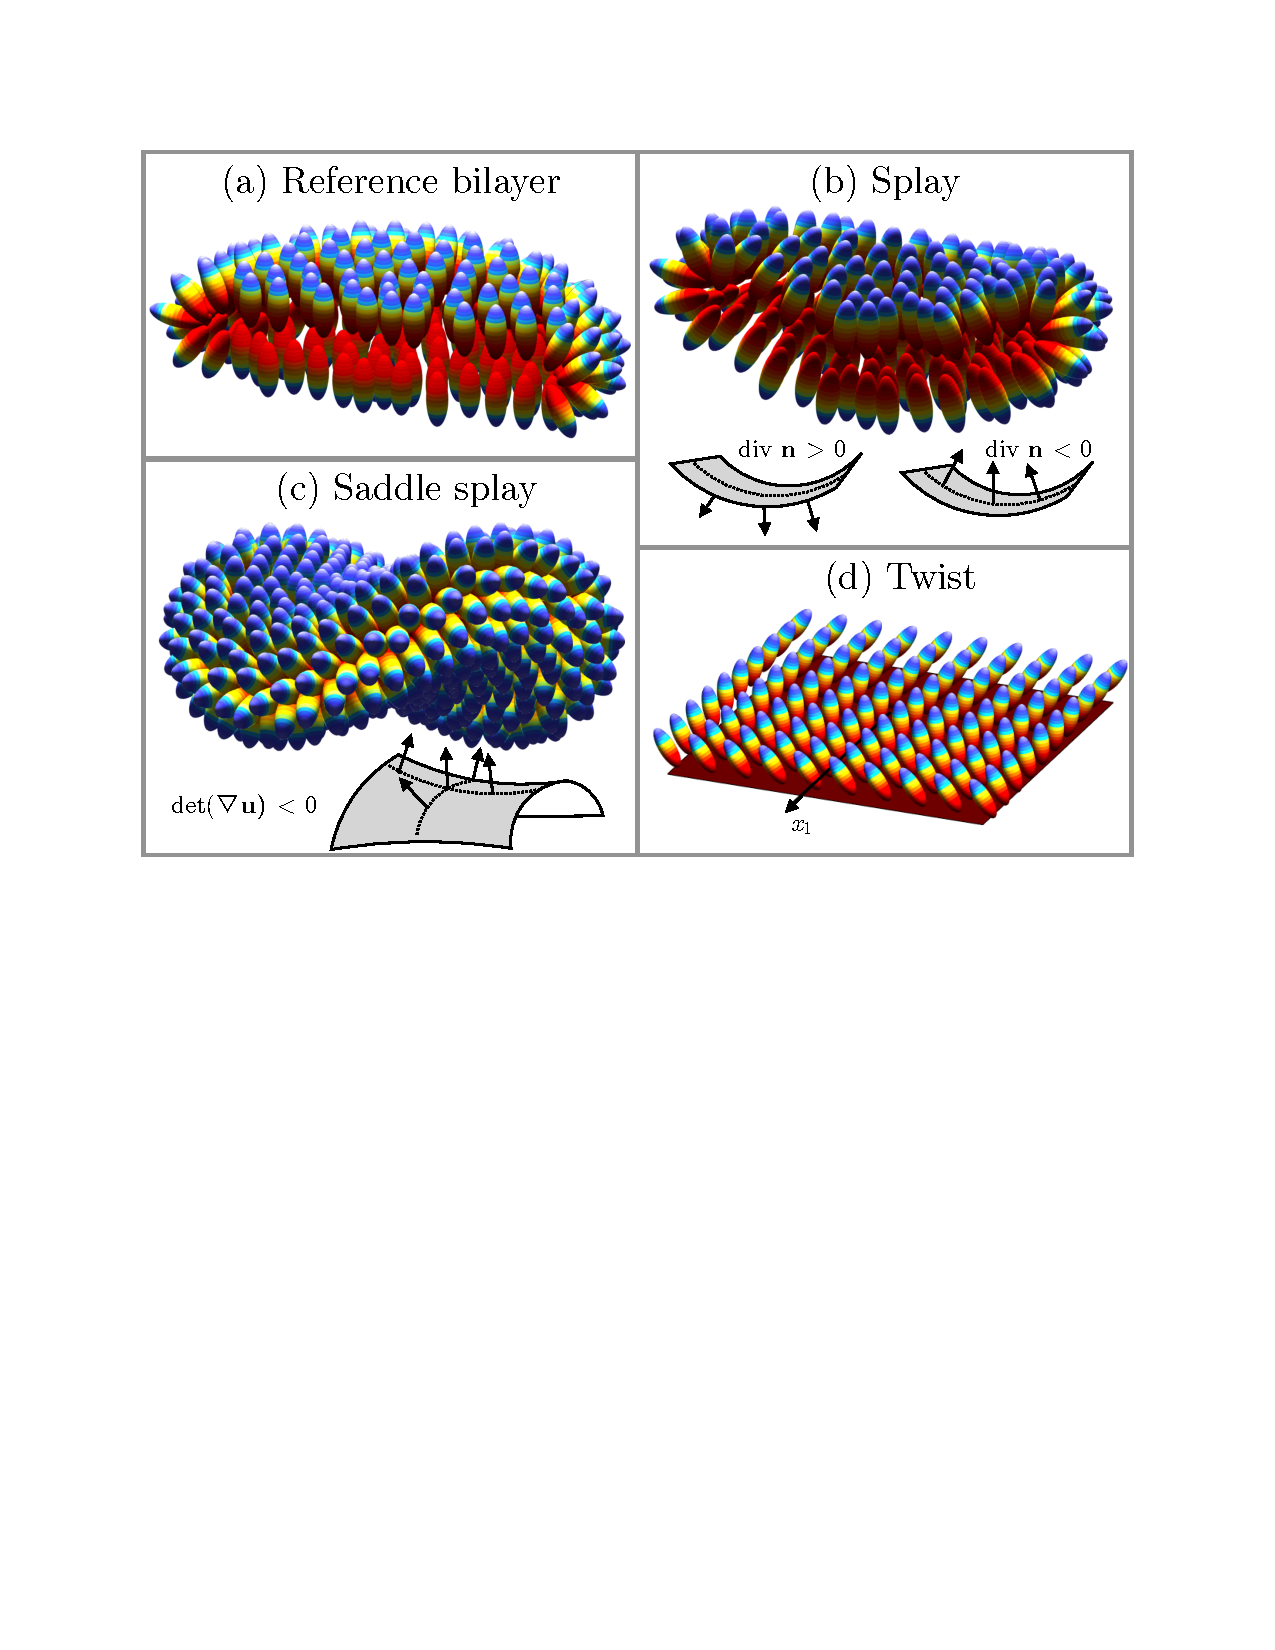
\includegraphics[width=0.46\textwidth]{Figures/Deformations.pdf}}
  \vspace{-5pt}
\caption{\label{fig:deformations} \footnotesize Sketch of the HK
 membrane model \cite{Hamm2000}.}
\end{wrapfigure}
%
This proposal will develop much-needed mathematical analysis to resolve
these controversies due to the assumptions in the HK theory. 


\sloppy
The HK framework assumes a three-dimensional lipid monolayer where the
internal structure consists of straight fibers that represent elongated
hydrocarbon chains.  The elastic energy density ${\cal W}$ is quadratic
in the Green-Lagrange strain tensor for this striated, internal
structure. This energy density decomposes into four, fundamental, and
independent deformations (Figure~\ref{fig:deformations}): splay ($\Div
{\bf n}$), twist ($\Curl {\bf n}$), saddle splay ($\det \nabla {\bf
n}$), and tilt ${\bf t}={\bf n}/({\bf N}\cdot {\bf n}) - {\bf N}$ where
${\bf N}$ is the unit surface normal;
\begin{equation}
\label{ansatz3}
{\cal W} \equiv \int_{\Sigma} 
  \tfrac{1}{2}\KB\left[ \left( \Div {\bf n} + k_0\right)^2 - k_0^2\right] 
+ \tfrac{1}{2}\KT (\Curl {\bf n})^2 + \KG  \det \nabla {\bf n} + \tfrac{1}{2}\KTH |{\bf t}|^2 \,dA.
\end{equation}
Here, the deformations come with elastic coefficients: the bending
modulus $\KB$, twist modulus $\KT$, saddle-splay modulus $\KG$, and tilt
modulus $\KTH$. The parameter $k_0$ is the spontaneous curvature and
determines the preferred lipid splay~\cite{RoLi15,Kozlov2007}.  

Although the HK elastic theory assumes small deformations, Galimzyanov
{\em et al.}~\cite{C9SM02079A} have shown that energies derived from
molecular dynamics and those derived from \eqref{ansatz3} are in
agreement, even when curvatures are large.  Under spatial scales much
larger than the membrane thickness, membrane energy is
well-characterized by the Canham-Helfrich energy used throughout the
fluid-structure literature \cite{QiangDu09, Lowengrub07,KimLai2010_JCP,
Hu, HuLaiSeolEtAl2016_JCP, qua-bir2014, qua-vee-you2019}. The
Canham-Helfrich energy is actually a special case of \eqref{ansatz3}
obtained by setting ${\bf n} =  \pm {\bf N}$ (the $\pm$ depending on
orientation) and collapsing both monolayers onto the membrane midplane.

\subsubsection{Simulations of the HAP model to estimate elastic moduli
and energy}
\begin{wrapfigure}[11]{r}{0.43\textwidth}
  \centerline{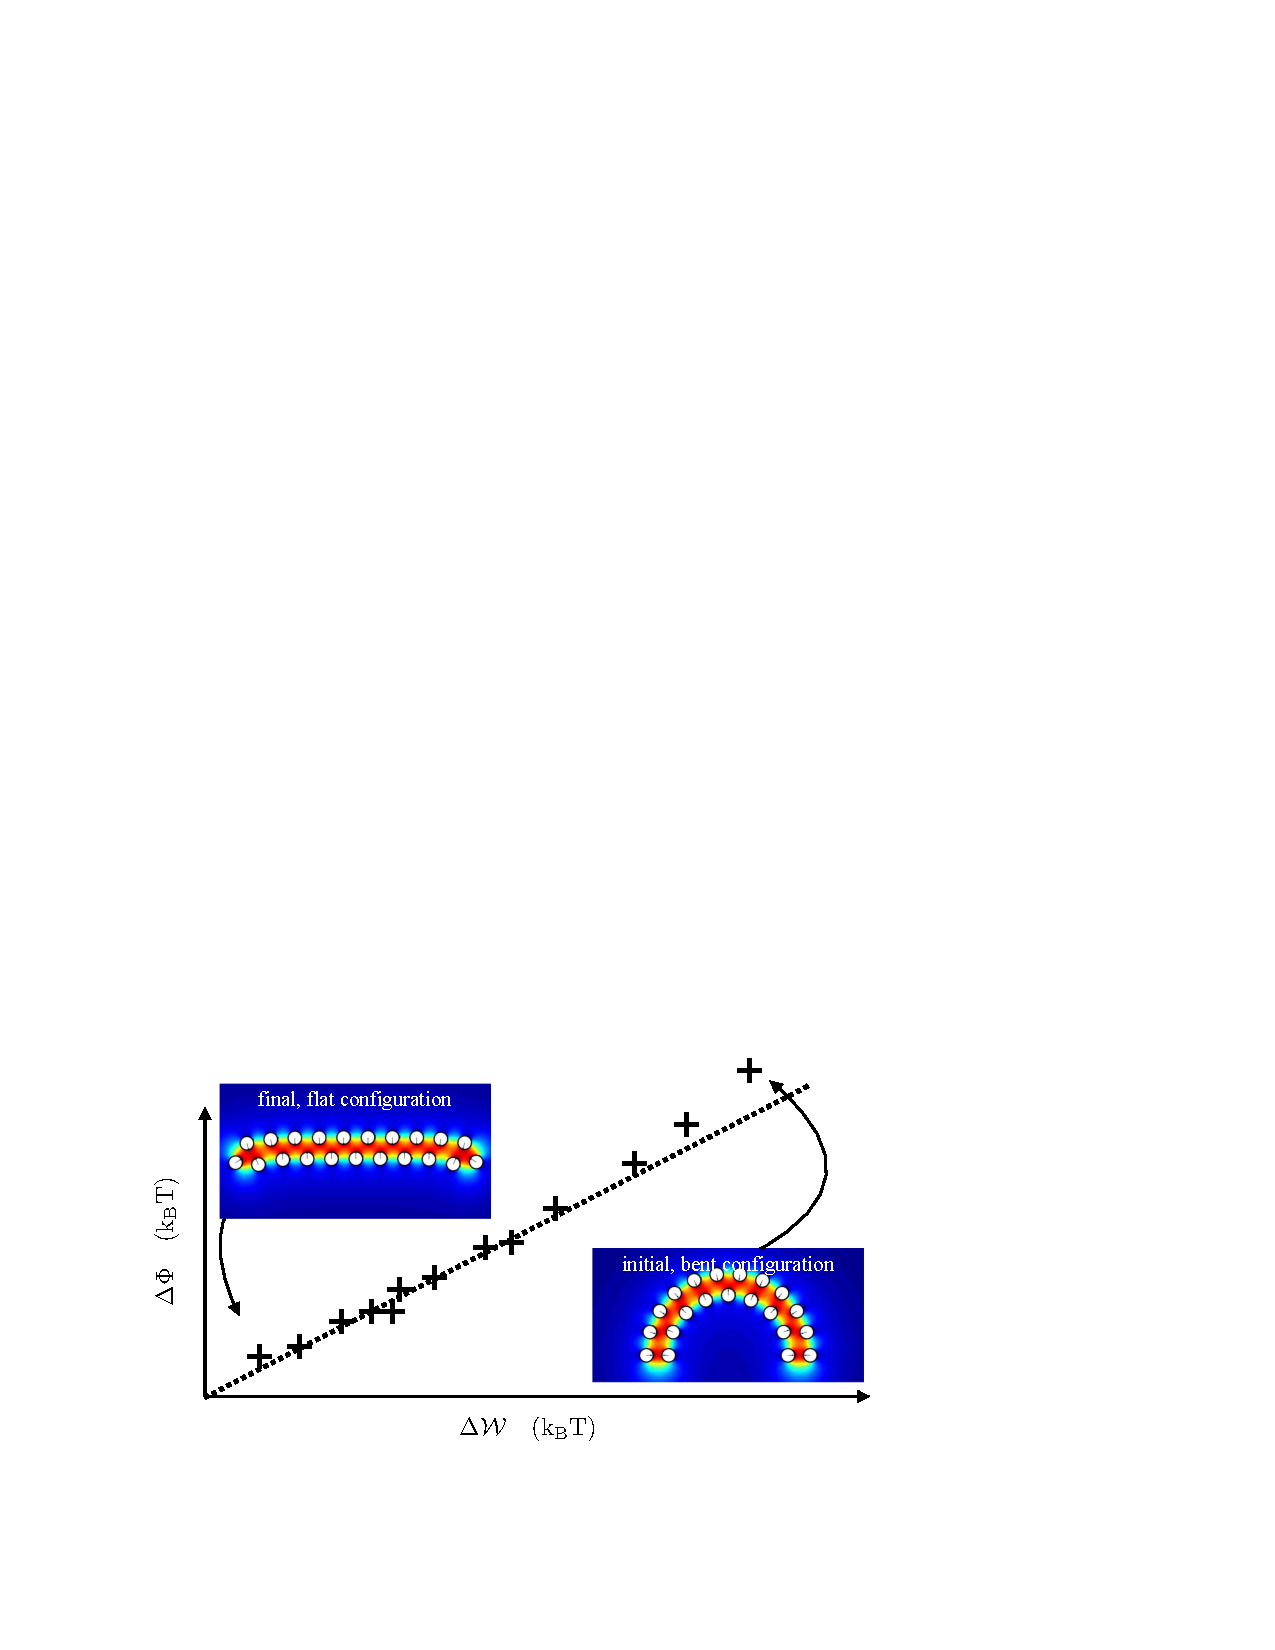
\includegraphics[width=0.42\textwidth]{Figures/Flattening.pdf}}
  \caption{\label{fig:flattening} \footnotesize Example of computing
  bending modulus of a lipid bilayer from particle simulation.}
\end{wrapfigure}
We propose to {\bf (i)} determine the value of effective elastic moduli
$\KB$, $\KT$, $\KG$, and $\KTH$ and then {\bf (ii)} understand how the
model parameters $\rho,$ $\gamma$, and the particle shape map onto
elastic moduli. An accurate and robust way to measure material
properties is to track the evolution of the bilayer as it relaxes from
an initially non-equilibrium
configuration~\cite{PhysRevLett.117.188102}.
Figure~\ref{fig:flattening} shows an example where the initial
configuration of a bilayer patch containing the splay deformation
without any other components (saddle splay, twist and tilt). As the bent
membrane flattens, both the self-interaction energy $\Phi$ and the
elastic energy ${\cal W}$ decrease, and because the saddle splay, twist,
and tilt stay zero, the slope gives the bending modulus in this case. 

Here we start with a particle-based bilayer in a specific
non-equilibrium shape that involves only one of the components of the
displacement in Figure~\ref{fig:deformations}, and then evolve the
particle system according to the time integration for \eqref{eq:stokes}.
Because elastic properties are independent of dissipation, we can forgo
solving for fluid velocity and set the translational velocity and
angular velocity directly proportional to the force and torque,
respectively. 

This yields a dissipation of the total potential \eqref{eq:total_poten},
which stabilizes the evolving bilayer shape.  Therefore, we reconstruct
an evolving monolayer dividing surface $\Sigma$ and director field ${\bf
n}$ by interpolating the particle centers and orientations. Using
\eqref{ansatz3}, we calculate a continuum energy $\mathcal{W}$ from the
interpolated shapes.

We propose to conduct calculations similar to the example of
Figure~\ref{fig:flattening} for other elastic moduli such as the
effective twist modulus $\KT$.  Molecular dynamics investigations find a
twist modulus about 1 \kBT~\cite{LeVeWa14}, and here, the specific
non-equilibrium shape consists of a single layer of amphiphilic
particles on a hydrophobic substrate as illustrated by
Figure~\ref{fig:deformations}D. Having a nonzero twist requires nonzero
tilt because the surface gradient of the lipid director equals the
second fundamental form whenever tilt is zero locally. The twist
deformation is a fully three-dimensional deformation.
\S\ref{subsec:specific_aim_3} addresses outstanding implementation
issues like three-dimensional boundary integral equation solvers.

The gradient descent technique is ineffective for measuring the saddle
splay modulus $\KG$ because the saddle splay energy is largely invariant
under shape changes.  To evaluate $\KG$, we will combine the present
particle simulations with the string method from PI RR's work on
membrane fusion \cite{RyKlYaCo16}. The string method is a numerical
scheme that finds least energy pathways separating energy basins
\cite{doi:10.1063/1.2720838}.  In the simplified Canham-Helfrich
formulation, saddle splay energy is an exact indicator of topological
transitions, thanks to the  Gauss-Bonnet theorem \cite{TerziDeserno17}.
More generally, PI RR has shown that saddle splay acts as a topological
indicator even in the presence of nonzero tilt \cite{RyKlYaCo16}.  As a
result, saddle splay can be quantified from the transition energies of a
least energy path of pore formation (Figure~\ref{fig:saddle_splay}).

The field of membrane continuum mechanics still lacks consensus as to
whether HK energy is the appropriate functional for bilayer energy.
\textbf{(i)} Researchers have assumed that $\KT = 0$ to effect lateral
fluidity in membranes~\cite{Hamm2000, TerziDeserno17, C9SM02079A,
PhysRevE.102.042406}. A value $\KT = 0$, however, makes~\eqref{ansatz3}
a noncoercive functional. \textbf{(ii)} Recently,~\cite{TerziDeserno17}
derived a tilt curvature term that was neglected from the HK
analysis~\cite{Hamm2000}.  Later,~\cite{C9SM02079A}
and~\cite{PhysRevE.102.042406} independently identified an inconsistency
in the argument used by~\cite{TerziDeserno17} arising from a transversal
tilt invariance assumption.  In~\cite{RyKlYaCo16}, PI RR and
collaborators showed that the tilt vector leads to unphysical cusps
depending on how one accounts for membrane thickness.  \textbf{(iii)}
Theoretical analysis of lipid phase transitions predict a negative
saddle-splay modulus around $-8$ \kBT~\cite{SIEGEL2004366,
SIEGEL20085200} that gives rise to a larger energy barrier for monolayer
fusion than is found by experiments~\cite{FrRoPi17, Tran7106,
TerziDeserno17}.
\begin{wrapfigure}[11]{l}{0.32\textwidth}
  \centerline{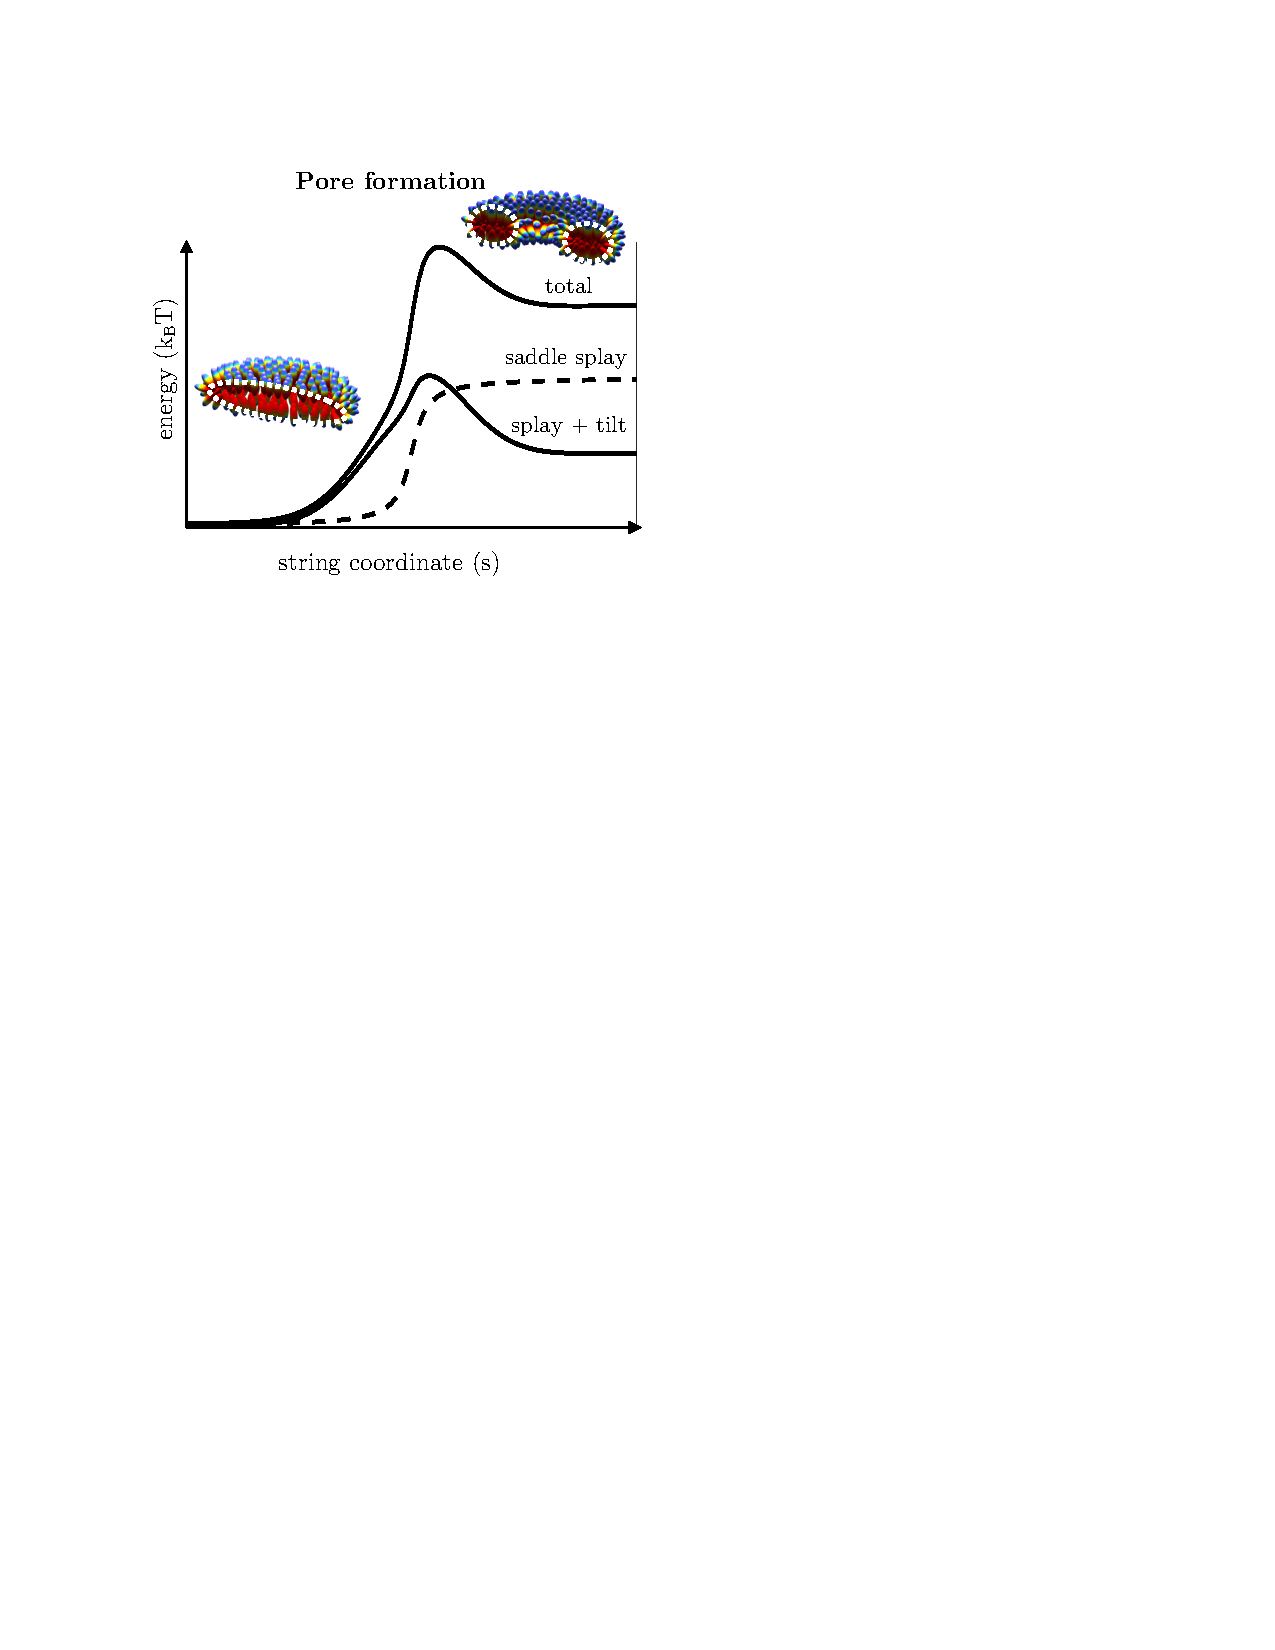
\includegraphics[width=0.31\textwidth]{Figures/SaddleSplayDiagram.pdf}}
  \caption{\label{fig:saddle_splay} \footnotesize Example of determining
  the saddle splay modulus.}
\end{wrapfigure}

The form of the elastic energy density~\eqref{ansatz3} is the same as
the Oseen-Frank energy density for nematic liquid
crystals~\cite{ANDRIENKO2018520, Tran7106, Helfrich73}. In fact, a lipid
monolayer acts as one layer in a smectic phase~\cite{REYESMATEO1995978,
Rangamani20140463, PhysRevLett.113.248102}. Based on this observation,
we propose to examine the HK analysis to resolve the aforementioned
inconsistencies. We will expand the strain tensor in terms of a plane
perpendicular to ${\bf n}$ (instead of the monolayer tangent plane as
done in the past works) so that the gradient terms in the elastic energy
completely decouple. Using this expansion we prove an exact identity
that gives the incompressibility condition by a Steiner-type polynomial
in $\Div {\bf n}$ and $\det \nabla {\bf n}$ \cite{Fe59}. In contrast,
the works~\cite{TerziDeserno17, PhysRevE.102.042406, Hamm2000,
C9SM02079A} utilize an approximate identity for incompressibility as a
base, so we can considerably improve upon the analysis of monolayer
energy.

\subsubsection{Analysis of the HAP model in terms of the HK functional}
The HK functional~\eqref{ansatz3} has transformed how scientists understand biological membranes, yet the
theory has received little attention in terms of
mathematical analysis. In the calculus of variations, the
principal question is whether a minimizer of an energy functional
exists. In the case of~\eqref{ansatz3}, the answer is presently unknown.
With regard to the simpler Canham-Helfrich energy,~\cite{Simon1993}
proved the existence of minimizing surfaces without boundary,
and~\cite{doi:10.1137/18M1195851} proved the well-posedness of a
spatially periodic, time-dependent elastic interface problem. An
analytical challenge for the HK functional~\eqref{ansatz3} is that
surface-director coupling makes it possible to have bounded energy
monolayers with corners, and such pathological examples must be ruled
out before carrying over the arguments for the Canham-Helfrich
functional to the present setting.

Our goal here is to develop tools that can explain functionals
like~\eqref{ansatz3} from first principles in terms of HAP. The
papers~\cite{doi:10.1063/5.0009734, Seguin2012, Seguin2014} give
statistical mechanical/mean field derivations of the Canham-Helfrich
energy from a pair-potential for rod-like molecules, but do not include
tilt, which is an indispensable deformation at biological scales. To
make progress, we must first understand how the HAP functional behaves
under various limits.

We first consider HAP in the limit of vanishing screening length. As a
concrete model problem, we consider a collection of colloidal polyhedral
where the binding energy of this system can be described by a discrete,
lower semicontinuous functional $\Phi_0$ whose value is the total
surface area of the polyhedra minus two times the area of any
overlapping faces. We conjecture that the $\Phi$ energy
$\Gamma$-converges to $\Phi_0$ \cite{Mugnai2013}, meaning that any
cluster points of minimizers of $\Phi$ converge to a minimum of $\Phi_0$
in the limit $\rho \to 0$. To address this conjecture, we employ
boundary layer analysis for the screened Laplace equation~\cite{Lee2018,
Lin2015, Shibata2004,1531-3492_2006_2_357, Lee2018}. The technique of
$\Gamma$-convergence is a powerful tool for numerical approximations and
with it we can help explain unexpected phenomena like hierarchical
self-assembly in colloidal systems~\cite{Luo2019}.

\end{comment}

